\chapter{Tecnologías Base del Proyecto}

\section{Tecnologías de localización y contexto}

La propuesta MuseIQ se apoya en un conjunto de tecnologías que permiten reconocer contexto espacial, sostener interacción accesible y responder consultas con soporte documental. En coherencia con los fundamentos expuestos en el Capítulo 6, el criterio rector no es la máxima sofisticación aislada de cada componente, sino la selección de tecnologías con costo contenido, disponibilidad operativa y capacidad suficiente para resolver el problema de mediación cultural presencial. Por ello, la base tecnológica del proyecto se organiza en tres grupos: localización y contexto, interacción con el visitante, e inteligencia y conocimiento.

\begin{figure}[!ht]
    \centering
    
\includegraphics[width=0.88\textwidth]{capas_tecnologicas_museiq.png}
    \caption[Capas tecnológicas base de MuseIQ]{Capas tecnológicas que sostienen la arquitectura base de MuseIQ.}
    \label{fig:capas-tecnologicas-museiq}
\end{figure}

\subsection{Bluetooth Low Energy (BLE) como base de proximidad}

Bluetooth Low Energy (BLE) constituye la tecnología principal para reconocimiento de proximidad en MuseIQ. Su pertinencia se explica por tres razones. En primer lugar, BLE permite difundir identificadores mediante advertising sin requerir procesos complejos de asociación o conexión persistente, lo que simplifica su uso en escenarios de visita libre. En segundo lugar, opera con consumo energético reducido, lo que favorece despliegues con balizas compactas y mantenimiento razonable. En tercer lugar, el ecosistema móvil actual dispone de soporte nativo para detección BLE, lo que hace viable una arquitectura BYOD centrada en el smartphone del visitante~\cite{leitch2023indoor,appleibeacon,googleeddystone}.

En un entorno museístico, la principal utilidad de BLE no consiste en estimar coordenadas exactas, sino en activar mediación situada. La literatura reciente sobre localización indoor confirma que BLE presenta ventajas de costo y despliegue frente a tecnologías más exigentes como UWB o Wi-Fi RTT, especialmente cuando el objetivo es reconocer cercanía relativa o presencia en una zona funcional~\cite{leitch2023indoor,qiao2024uwb}. Esta característica se alinea directamente con MuseIQ, donde la variable relevante es la sala o zona probable de observación, no la ubicación centimétrica del visitante.

\begin{figure}[!ht]
    \centering
    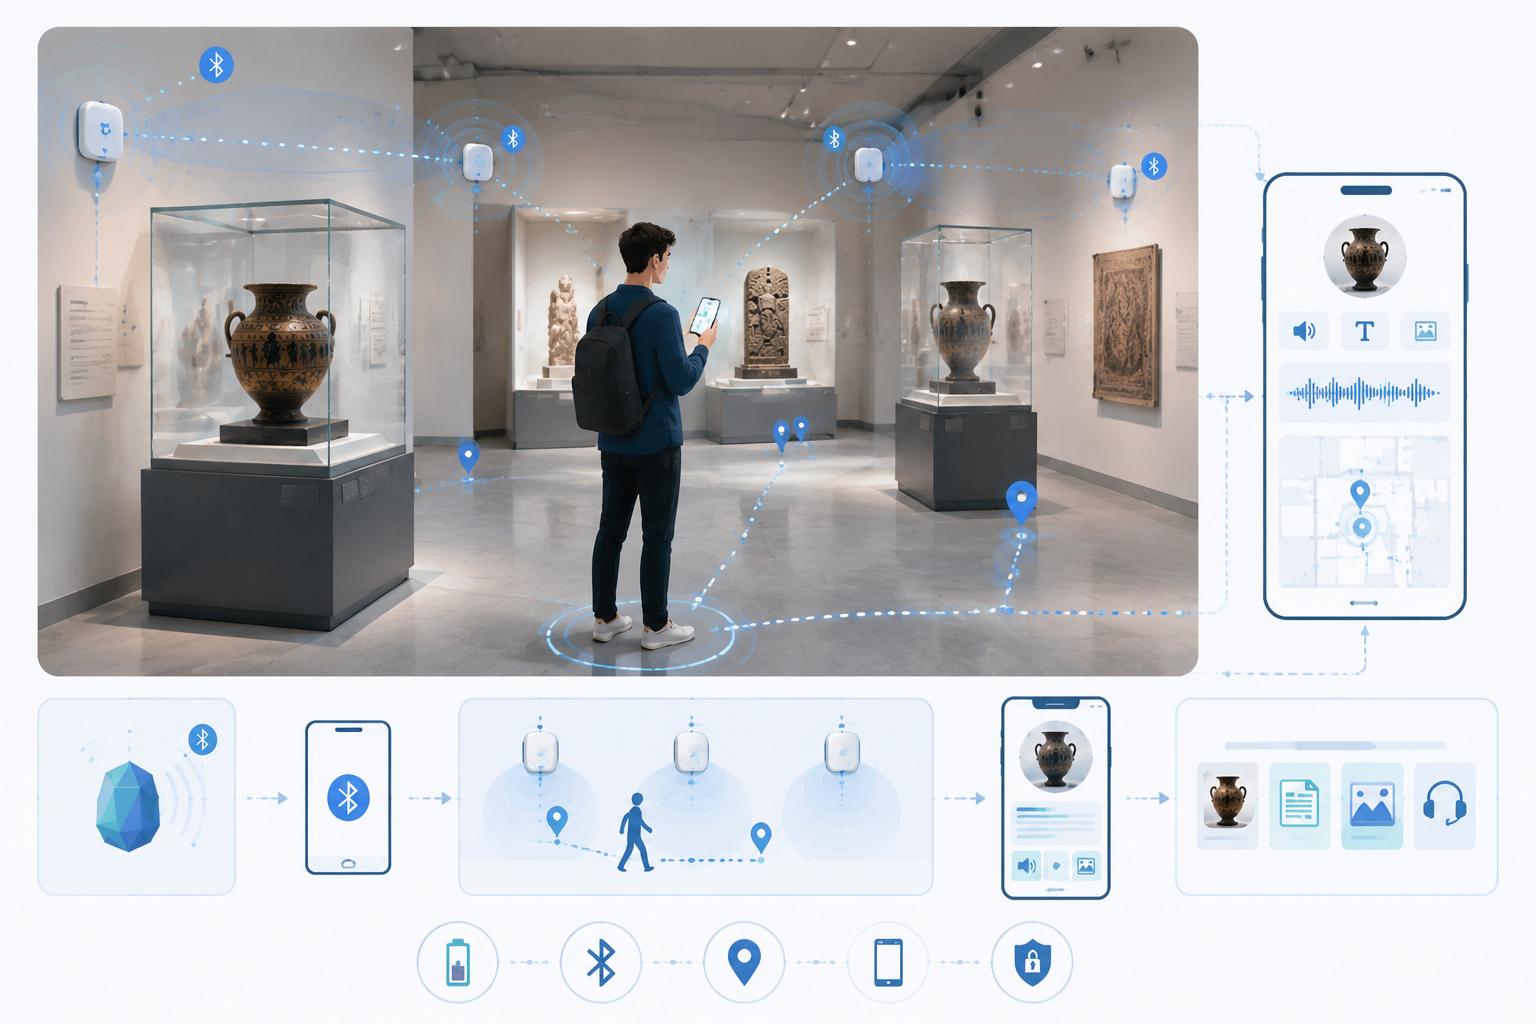
\includegraphics[width=0.92\textwidth]{src/imgs/07/ble-base-proximidad.png}
    \caption[BLE como base de proximidad en MuseIQ]{Representación conceptual del uso de Bluetooth Low Energy como tecnología de proximidad para reconocer la zona probable del visitante dentro del museo. Fuente: elaboración propia con apoyo de generación asistida por IA.}
    \label{fig:ble-base-proximidad}
\end{figure}

La Figura~\ref{fig:ble-base-proximidad} resume esta lógica de operación: las balizas distribuidas en el entorno emiten señales de proximidad que el smartphone puede detectar para inferir el contexto espacial más probable del usuario y activar contenido pertinente durante la visita.

\subsection{Beacons y uso de ESP32}

La infraestructura de proximidad propuesta para MuseIQ se implementa mediante beacons basados en ESP32. Un beacon puede entenderse como un emisor que transmite periódicamente paquetes BLE con identificadores o metadatos mínimos, de modo que el smartphone pueda detectar qué punto del entorno se encuentra más próximo. La elección de ESP32 responde a criterios de integración, accesibilidad económica y versatilidad de prototipado. Se trata de una plataforma ampliamente disponible, con soporte oficial para Bluetooth Low Energy y con bibliotecas suficientemente maduras para configurar esquemas de advertising compatibles con arquitecturas de proximidad~\cite{espressifibeacon,espressif2026esp32}.

Desde el punto de vista del proyecto, el uso de ESP32 aporta una ventaja adicional: permite construir una infraestructura incremental. Es posible desplegar beacons por sala, módulo o zona, calibrar potencia e intervalo de emisión, y ampliar cobertura por etapas sin rediseñar el sistema completo. Esta lógica resulta particularmente adecuada para museos públicos o instituciones con restricciones presupuestales, donde la implementación progresiva es preferible a soluciones que exigen inversión integral desde el inicio.

\begin{figure}[!ht]
    \centering
    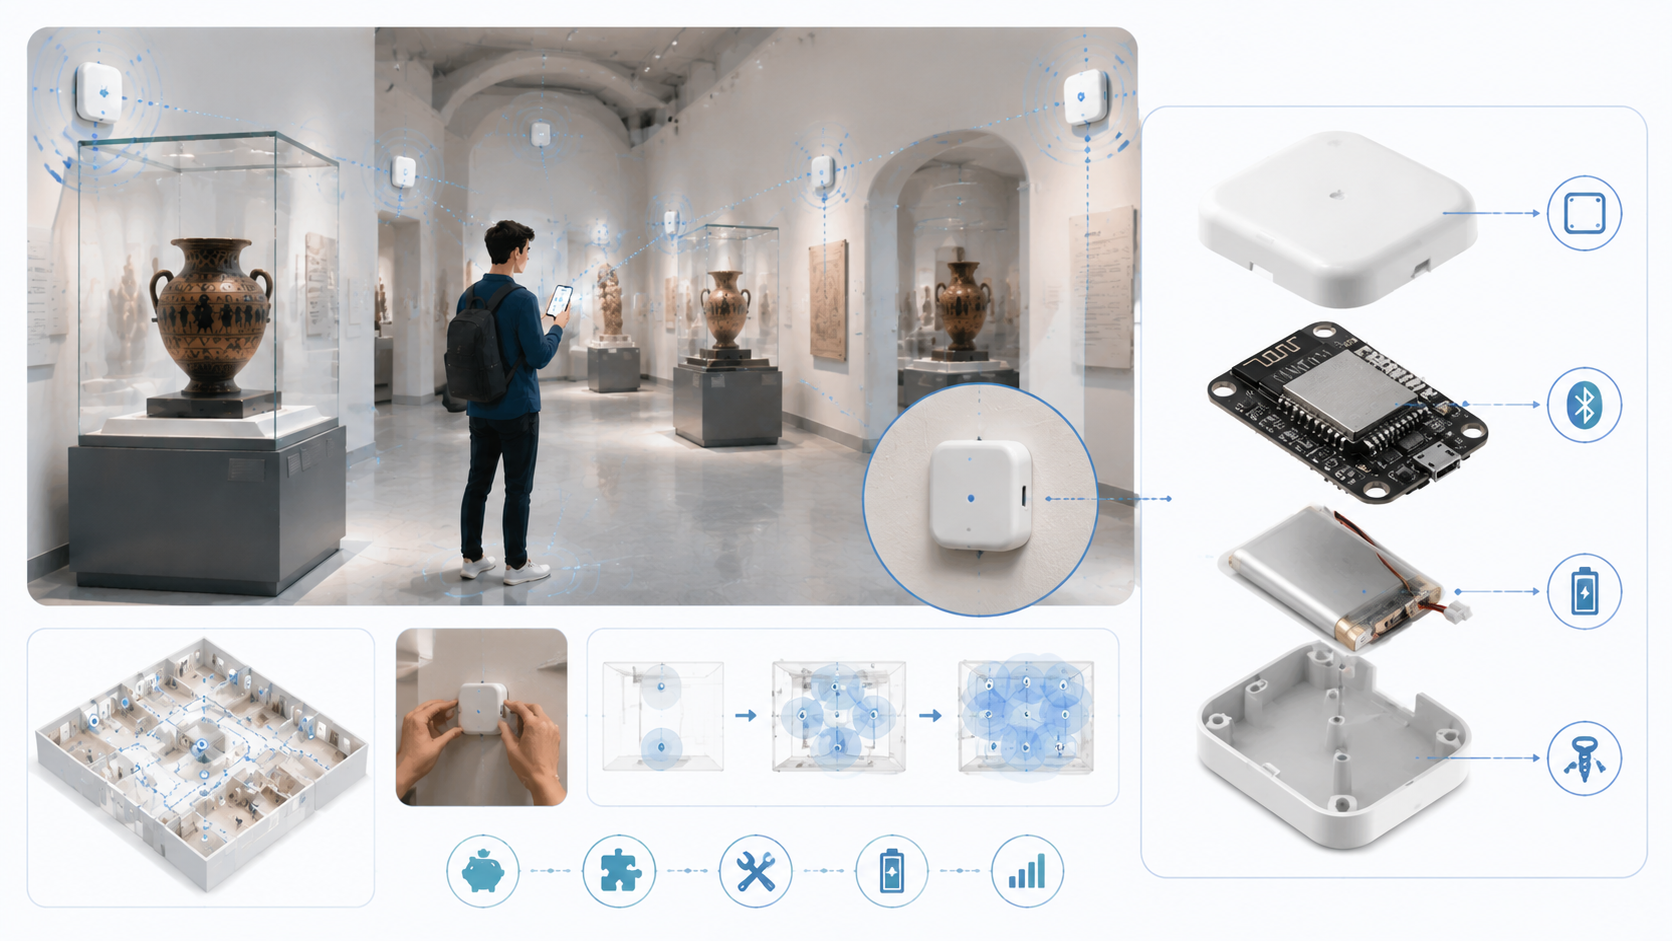
\includegraphics[width=0.92\textwidth]{src/imgs/07/beacons-esp32.png}
    \caption[Beacons basados en ESP32 para MuseIQ]{Esquema visual del despliegue de beacons basados en ESP32 en salas y vitrinas del museo como infraestructura de proximidad de bajo costo. Fuente: elaboración propia con apoyo de generación asistida por IA.}
    \label{fig:beacons-esp32}
\end{figure}

Como muestra la Figura~\ref{fig:beacons-esp32}, la incorporación de ESP32 permite imaginar una red ligera de balizas distribuida por zonas, compatible con estrategias de implementación progresiva y mantenimiento razonable.

\subsection{RSSI y reconocimiento funcional por sala o zona}

La señal recibida de un beacon BLE puede interpretarse mediante el indicador RSSI (\textit{Received Signal Strength Indicator}), utilizado como aproximación a cercanía relativa. Aunque RSSI es sensible a interferencias, orientación del dispositivo, obstáculos físicos y heterogeneidad de receptores, sigue siendo útil cuando se adopta una granularidad funcional y no geométrica. En MuseIQ, RSSI no se emplea para calcular distancias exactas, sino para inferir cuál es la sala o zona de mayor probabilidad, lo que basta para activar contenido contextual pertinente~\cite{verde2023blemuseum,leitch2023indoor}.

Esta decisión metodológica es importante porque convierte una limitación técnica en una ventaja de diseño. En vez de perseguir un esquema de posicionamiento de alta precisión, costoso y más frágil operativamente, MuseIQ aprovecha RSSI como parte de una lógica robusta de reconocimiento por sala. El estudio de Verde et al. en un museo real refuerza esta elección, al demostrar que una solución BLE basada en RSSI puede sostener identificación funcional de sala y entrega de contenido contextual en condiciones de operación museística~\cite{verde2023blemuseum}.

\begin{figure}[!ht]
    \centering
    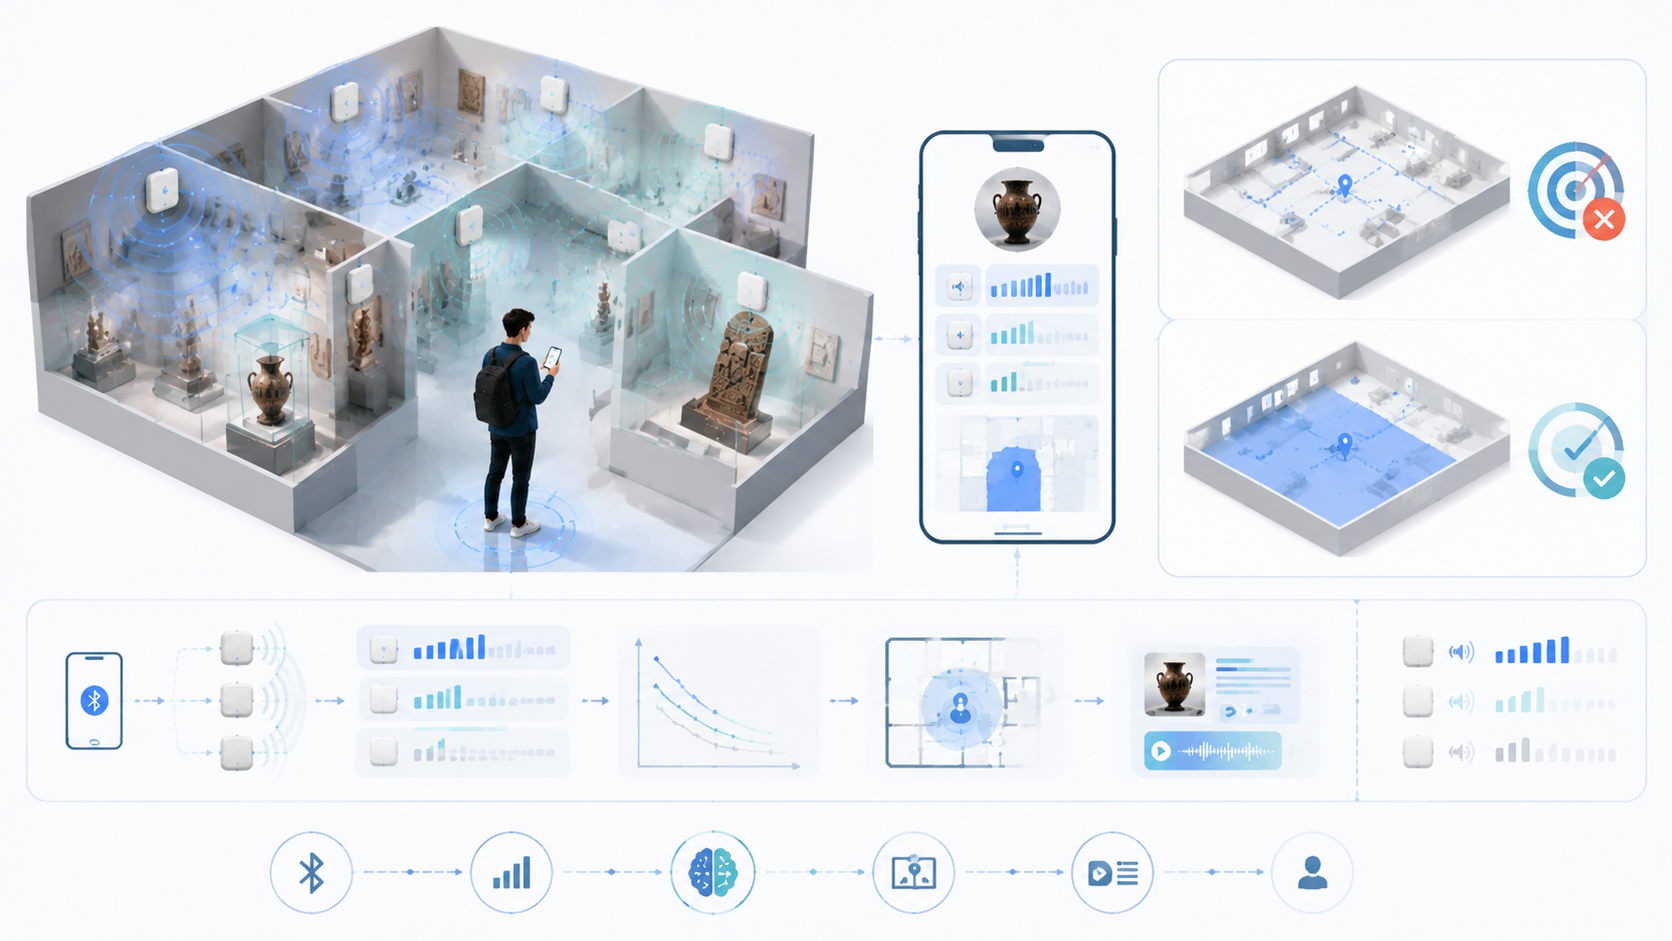
\includegraphics[width=0.92\textwidth]{src/imgs/07/rssi-reconocimiento-sala.png}
    \caption[Reconocimiento funcional por sala mediante RSSI]{Visualización del uso de la intensidad de señal RSSI para determinar la sala o zona de mayor probabilidad, privilegiando reconocimiento funcional sobre precisión centimétrica. Fuente: elaboración propia con apoyo de generación asistida por IA.}
    \label{fig:rssi-reconocimiento-sala}
\end{figure}

La Figura~\ref{fig:rssi-reconocimiento-sala} ilustra precisamente esta interpretación: el sistema compara intensidades relativas de señal para decidir cuál es el contexto espacial más plausible y, a partir de ello, orientar la mediación digital.

\subsection{Sensores del smartphone para orientación y contexto}

La capa de contexto no depende exclusivamente de BLE. MuseIQ incorpora también sensores del smartphone, especialmente aquellos relacionados con posición y orientación del dispositivo. La documentación oficial de Android describe mecanismos para inferir orientación combinando acelerómetro y sensor geomagnético, lo que permite estimar azimuth, pitch y roll como variables complementarias para interpretar hacia dónde se dirige o enfoca el visitante~\cite{android2026positionsensors}.

En términos funcionales, esta información reduce ambigüedad contextual. BLE puede sugerir la sala probable, pero no necesariamente el foco de observación dentro de esa sala. La orientación del dispositivo, aun con ruido e imprecisión, puede apoyar decisiones como priorizar contenido de la vitrina o pieza hacia la que aparentemente se dirige el usuario, o bien mejorar consistencia al combinarse con historial reciente de detecciones. Así, los sensores del teléfono cumplen un rol auxiliar en la construcción de contexto y fortalecen la pertinencia de la respuesta del sistema.

\begin{figure}[!ht]
    \centering
    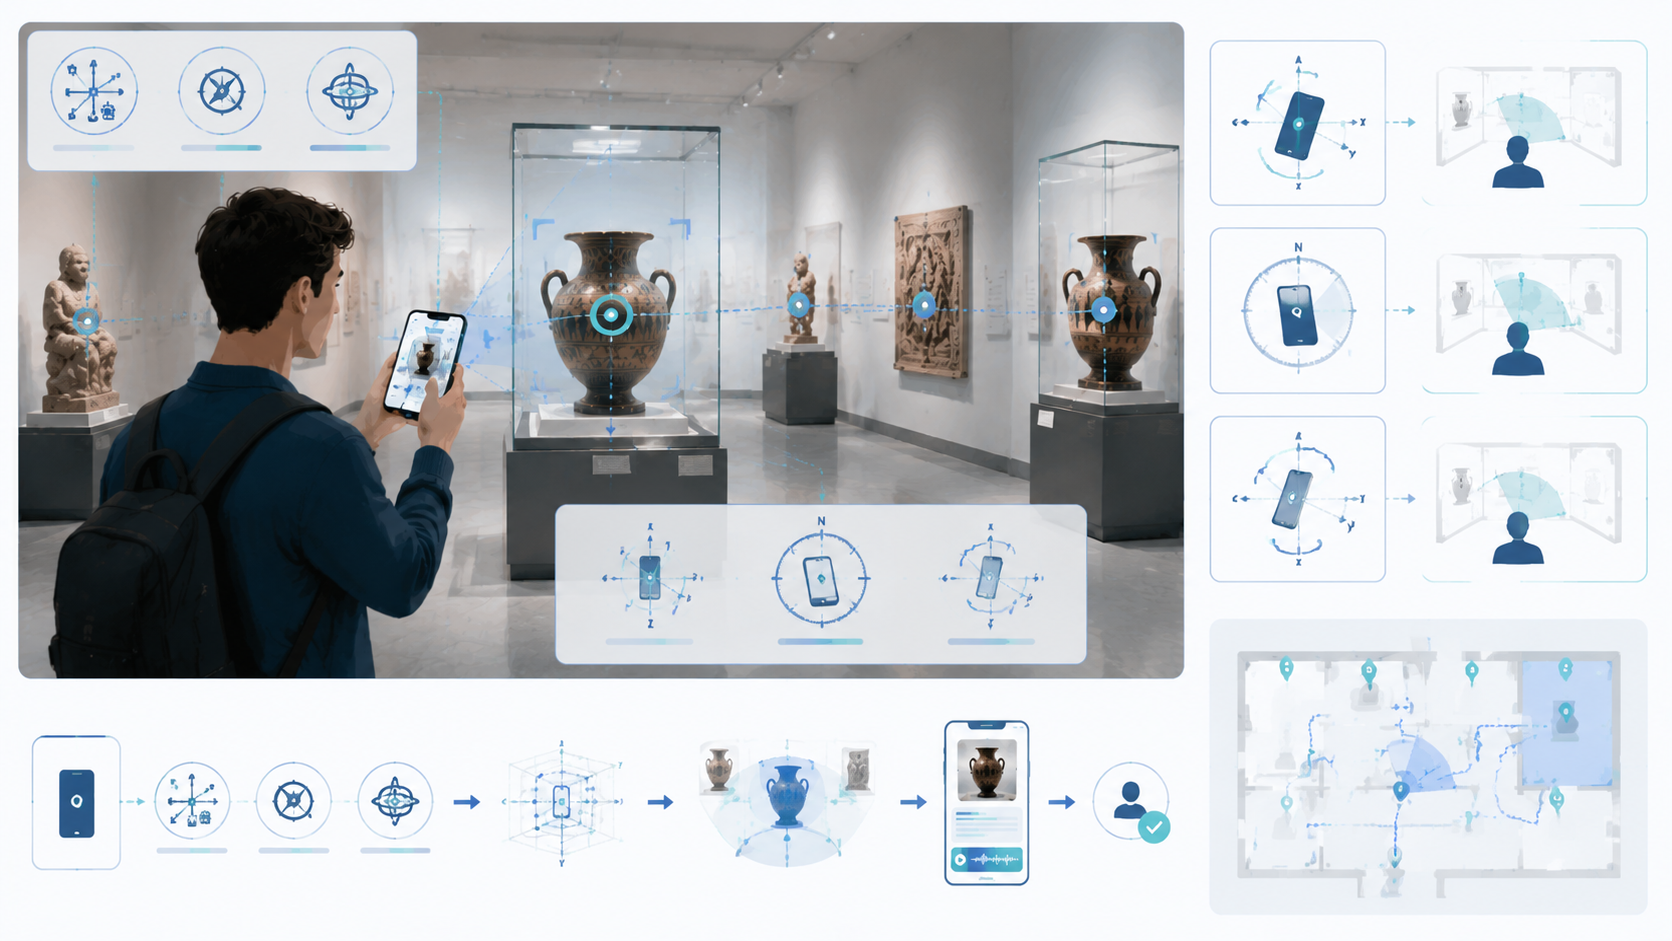
\includegraphics[width=0.92\textwidth]{src/imgs/07/sensores-smartphone-orientacion.png}
    \caption[Sensores del smartphone para orientación contextual]{Representación del uso de sensores del smartphone para estimar orientación del dispositivo y complementar la inferencia de contexto durante la visita. Fuente: elaboración propia con apoyo de generación asistida por IA.}
    \label{fig:sensores-smartphone-orientacion}
\end{figure}

En la Figura~\ref{fig:sensores-smartphone-orientacion} se observa cómo la orientación del teléfono añade una capa interpretativa adicional que ayuda a reducir ambigüedad entre piezas cercanas dentro de una misma sala.

\section{Tecnologías de interacción con el visitante}

\subsection{Smartphone como plataforma base BYOD}

MuseIQ adopta un enfoque \textit{Bring Your Own Device} (BYOD), en el que el visitante utiliza su propio smartphone como plataforma de interacción. Desde el punto de vista tecnológico, esta decisión permite concentrar en un solo dispositivo las capacidades mínimas requeridas por el sistema: detección BLE, lectura de sensores, captura de voz, reproducción de audio y visualización de contenido. De este modo, la aplicación puede operar sobre una plataforma ya disponible para el usuario sin requerir terminales especializados por parte del museo.

El contexto nacional refuerza esta decisión: la alta penetración de smartphones en hogares peruanos brinda una base realista para implementar experiencias de mediación digital apoyadas en el dispositivo personal del visitante~\cite{osiptel2024smartphone}. No obstante, el enfoque BYOD también impone restricciones técnicas relevantes, como heterogeneidad de hardware, diferencias entre versiones del sistema operativo, gestión de permisos y variabilidad en sensores y rendimiento. Por ello, su elección no solo responde a disponibilidad, sino también a la necesidad de diseñar una solución robusta frente a esa diversidad de dispositivos.

\begin{figure}[!ht]
    \centering
    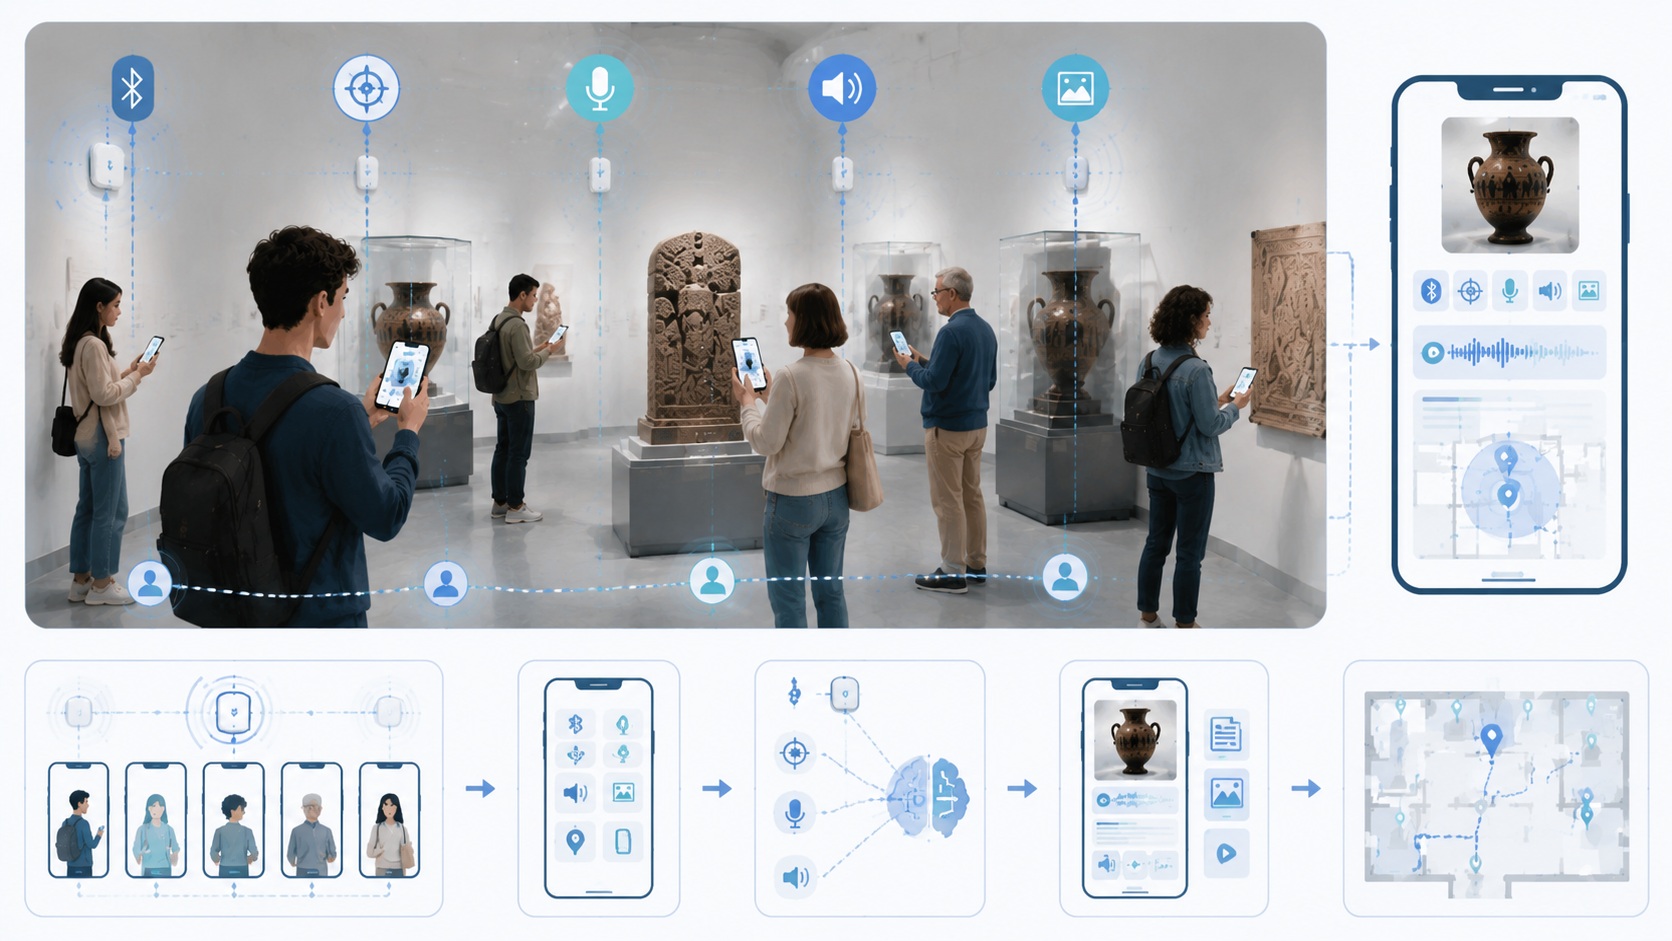
\includegraphics[width=0.92\textwidth]{src/imgs/07/smartphone-byod.png}
    \caption[Smartphone como plataforma BYOD en MuseIQ]{Representación del enfoque Bring Your Own Device, en el que el smartphone del visitante concentra las funciones principales de interacción con el sistema. Fuente: elaboración propia con apoyo de generación asistida por IA.}
    \label{fig:smartphone-byod}
\end{figure}

La Figura~\ref{fig:smartphone-byod} sintetiza esta decisión de diseño: el teléfono personal no actúa solo como pantalla, sino como plataforma integrada de detección, interacción y acceso al contenido contextual.

\subsection{Tecnologías de voz: TTS y STT}

La interacción por voz constituye otra tecnología base del proyecto. MuseIQ incorpora síntesis de voz (\textit{Text-to-Speech}, TTS) para convertir contenido textual en salida auditiva, y reconocimiento de voz (\textit{Speech-to-Text}, STT) para capturar consultas habladas del visitante. Esta combinación no se incluye como accesorio, sino como mecanismo funcional para accesibilidad, fluidez de uso y acompañamiento durante recorridos presenciales. La investigación de Wang muestra precisamente que las guías por voz en museos mejoran autonomía y accesibilidad, especialmente para usuarios que enfrentan barreras de lectura sostenida o requieren interacción más natural~\cite{wang2024voiceguide}.

Desde el punto de vista tecnológico, Android ofrece soporte nativo tanto para TTS como para reconocimiento de voz, lo que facilita la incorporación de estas capacidades sobre la misma plataforma móvil empleada por MuseIQ~\cite{android2026tts,android2026speech}. Esto hace posible una experiencia multimodal donde el visitante puede escuchar explicaciones, formular preguntas habladas y recibir respuestas sin abandonar el recorrido ni depender enteramente de interacción táctil.

\begin{figure}[!ht]
    \centering
    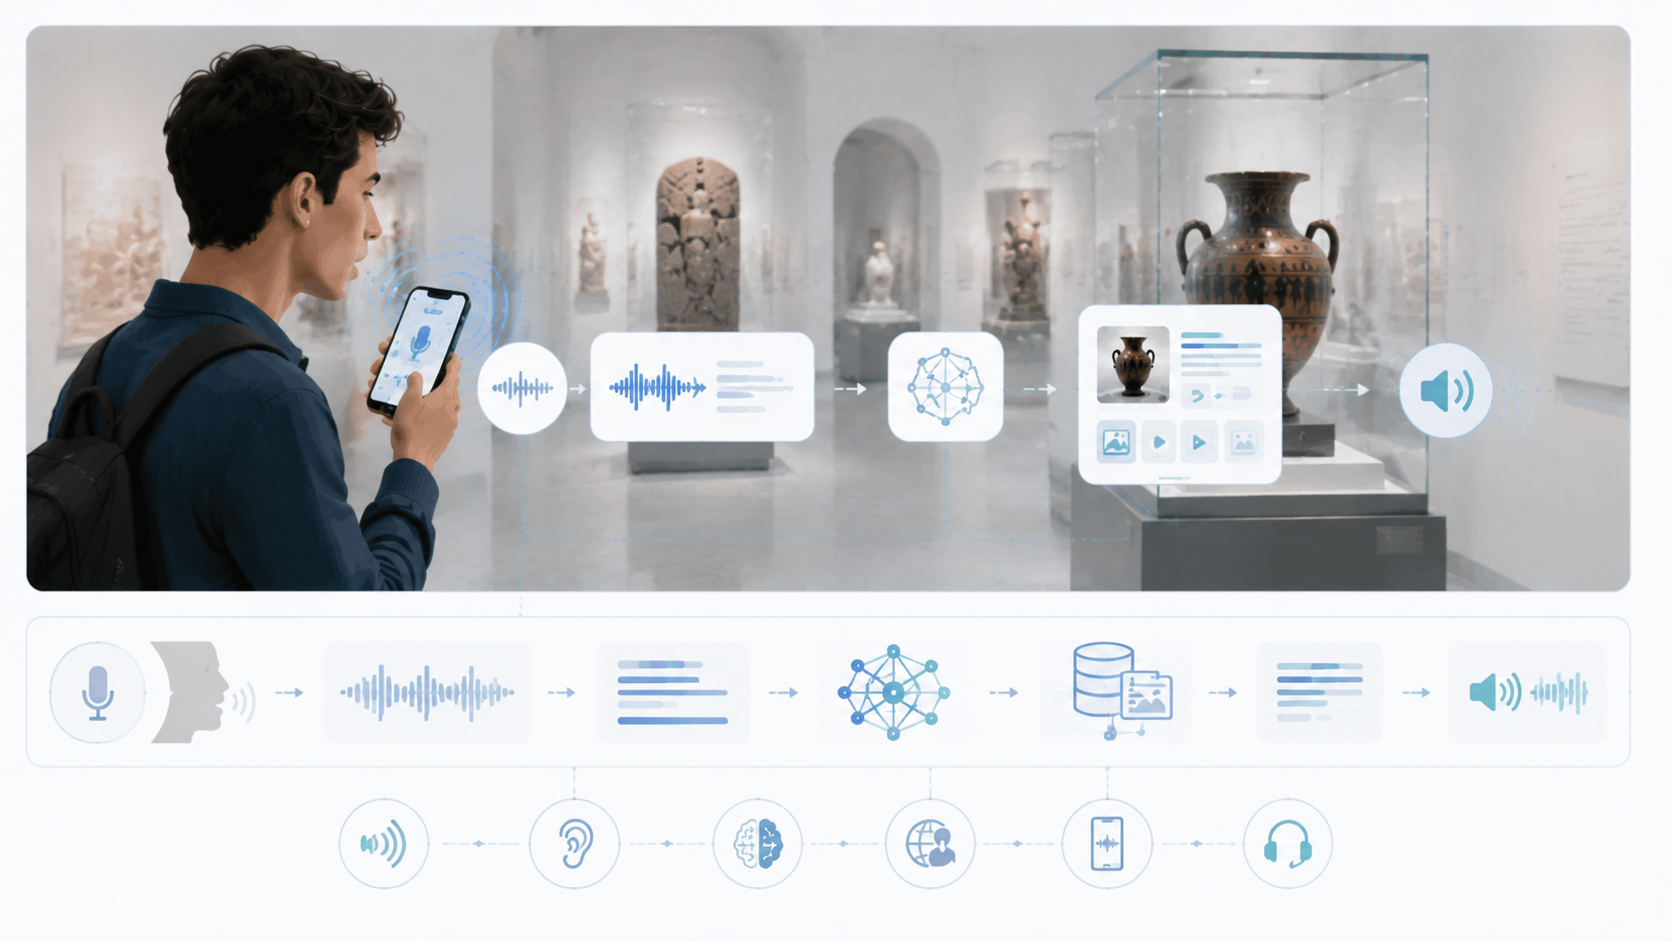
\includegraphics[width=0.92\textwidth]{src/imgs/07/tts-stt.png}
    \caption[Tecnologías de voz TTS y STT en MuseIQ]{Esquema conceptual de la interacción por voz en MuseIQ, integrando reconocimiento de habla y síntesis de voz durante la visita museística. Fuente: elaboración propia con apoyo de generación asistida por IA.}
    \label{fig:tts-stt}
\end{figure}

La Figura~\ref{fig:tts-stt} resume el ciclo de interacción por voz previsto en la propuesta: el visitante formula una consulta hablada, el sistema la interpreta y devuelve una respuesta en formato audible sin interrumpir el recorrido.

\subsection{Interacción multimodal en la visita museística}

La multimodalidad es una propiedad central de la propuesta. MuseIQ no depende de un único canal de interacción, sino que articula texto, audio, voz y contexto espacial. Esta decisión es particularmente adecuada para un museo, donde el visitante alterna entre observar piezas, desplazarse, escuchar explicaciones y formular preguntas espontáneas. Desde una perspectiva de diseño, la multimodalidad también incrementa robustez: si el ambiente es ruidoso, el sistema puede privilegiar salida textual; si el visitante prefiere no leer, TTS sostiene la mediación; y si se requiere exploración más abierta, la consulta por voz reduce fricción respecto a interfaces rígidas o excesivamente jerárquicas.

En consecuencia, la capa de interacción se entiende como un sistema adaptativo de acceso al contenido, no simplemente como una interfaz gráfica móvil. Esta visión mantiene coherencia con la idea de mediación cultural digital situada ya desarrollada en capítulos previos.

\begin{figure}[!ht]
    \centering
    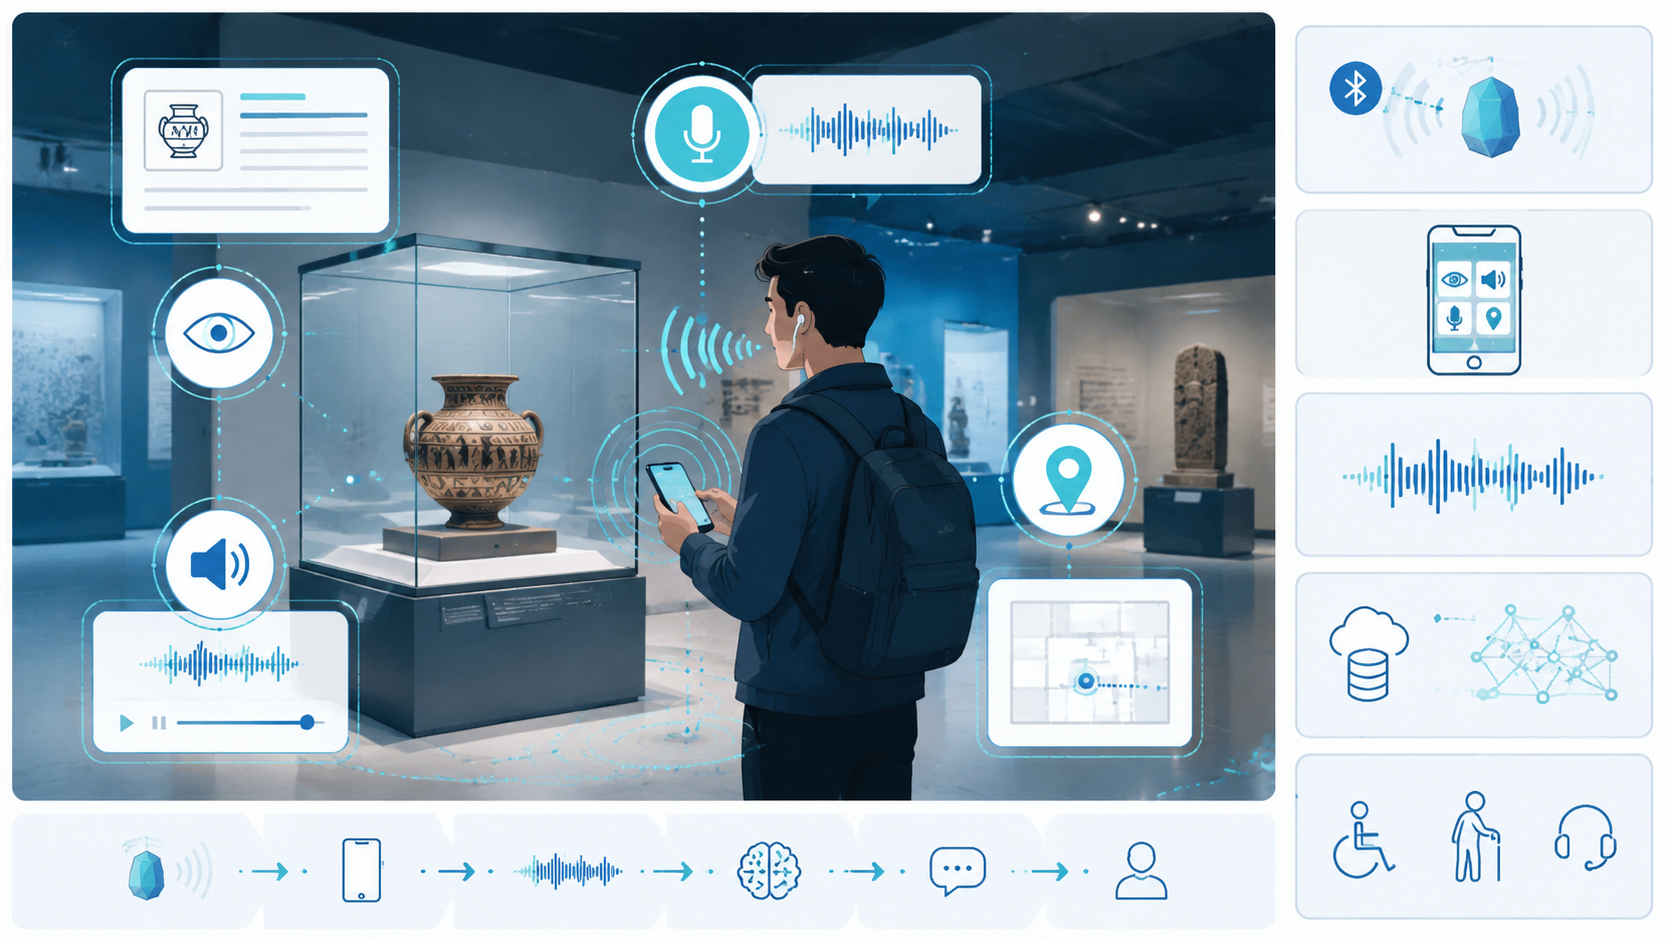
\includegraphics[width=0.92\textwidth]{src/imgs/07/interaccion-multimodal.png}
    \caption[Interacción multimodal durante la visita museística]{Representación de la articulación entre texto, audio, voz y contexto espacial como base de una experiencia de visita multimodal. Fuente: elaboración propia con apoyo de generación asistida por IA.}
    \label{fig:interaccion-multimodal}
\end{figure}

Como se aprecia en la Figura~\ref{fig:interaccion-multimodal}, la multimodalidad no se limita a superponer canales, sino que busca ofrecer distintas rutas de acceso al mismo contenido según la situación de uso del visitante.

\section{Tecnologías de inteligencia y conocimiento}

\subsection{Modelos de lenguaje y capacidad conversacional}

La base inteligente de MuseIQ se apoya en modelos de lenguaje modernos, cuya arquitectura dominante deriva de los Transformers. El trabajo fundacional de Vaswani et al. demostró que los mecanismos de atención permiten modelar dependencias en secuencias sin recurrencia explícita, habilitando mejoras significativas en procesamiento de lenguaje natural y abriendo el camino a los modelos conversacionales contemporáneos~\cite{vaswani2017attention}. Para MuseIQ, esto resulta relevante porque permite interpretar consultas abiertas y formular respuestas naturales sobre contenidos curatoriales.

Sin embargo, el proyecto no requiere un modelo de lenguaje entendido como generador libre de texto, sino como interfaz flexible para dialogar sobre conocimiento institucional. La pertinencia de esta tecnología radica en que el visitante puede formular preguntas variadas, con distintos niveles de detalle y vocabulario, sin depender de menús rígidos o rutas lineales predefinidas. Así, el modelo de lenguaje actúa como capa de comprensión y redacción, facilitando una mediación más natural y personalizada.

\begin{figure}[!ht]
    \centering
    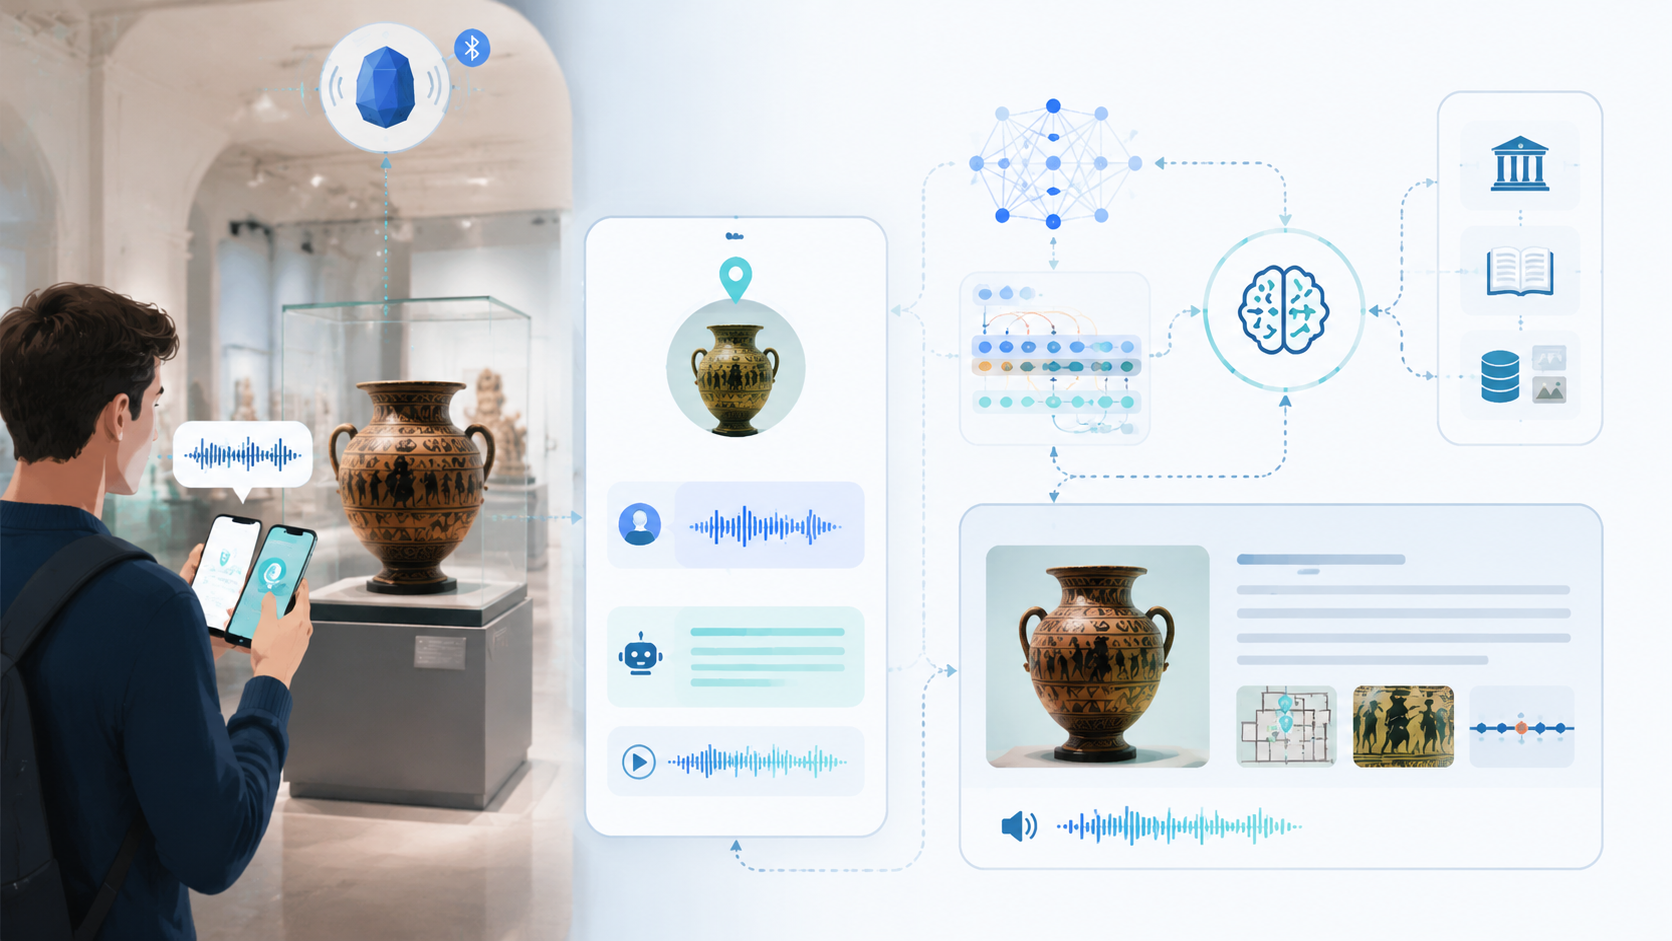
\includegraphics[width=0.92\textwidth]{src/imgs/07/modelos-lenguaje-conversacional.png}
    \caption[Modelos de lenguaje y capacidad conversacional]{Representación de los modelos de lenguaje como interfaz conversacional capaz de interpretar preguntas abiertas y formular respuestas naturales en contexto museístico. Fuente: elaboración propia con apoyo de generación asistida por IA.}
    \label{fig:modelos-lenguaje-conversacional}
\end{figure}

La Figura~\ref{fig:modelos-lenguaje-conversacional} permite visualizar este papel de la inteligencia lingüística como mediadora entre la consulta libre del visitante y la formulación de una respuesta comprensible y contextualizada.

\subsection{Recuperación aumentada de información (RAG)}

Una limitación crítica de los modelos de lenguaje es la posibilidad de producir respuestas plausibles pero incorrectas o no verificables. En dominios patrimoniales, esta limitación es especialmente sensible, ya que el contenido debe respetar criterios curatoriales, trazabilidad institucional y fidelidad interpretativa. Por ello, MuseIQ incorpora Retrieval-Augmented Generation (RAG) como tecnología base para la capa inteligente. El enfoque RAG combina recuperación de información desde una memoria externa con generación condicionada, de modo que la respuesta se apoye en fragmentos documentales recuperados del corpus pertinente~\cite{lewis2020rag}.

La relevancia de RAG para MuseIQ es directa: permite anclar la conversación a fichas, descripciones curatoriales, textos de sala o documentación institucional, reduciendo alucinaciones y mejorando consistencia semántica. Además, trabajos recientes sobre reducción de alucinación mediante recuperación aumentada refuerzan la utilidad de este paradigma en sistemas que requieren salidas más controladas y estructuradas~\cite{bechard2024hallucination}. En consecuencia, la inteligencia de MuseIQ no se concibe como una generación abierta, sino como una conversación guiada por evidencia documental recuperada.

\begin{figure}[!ht]
    \centering
    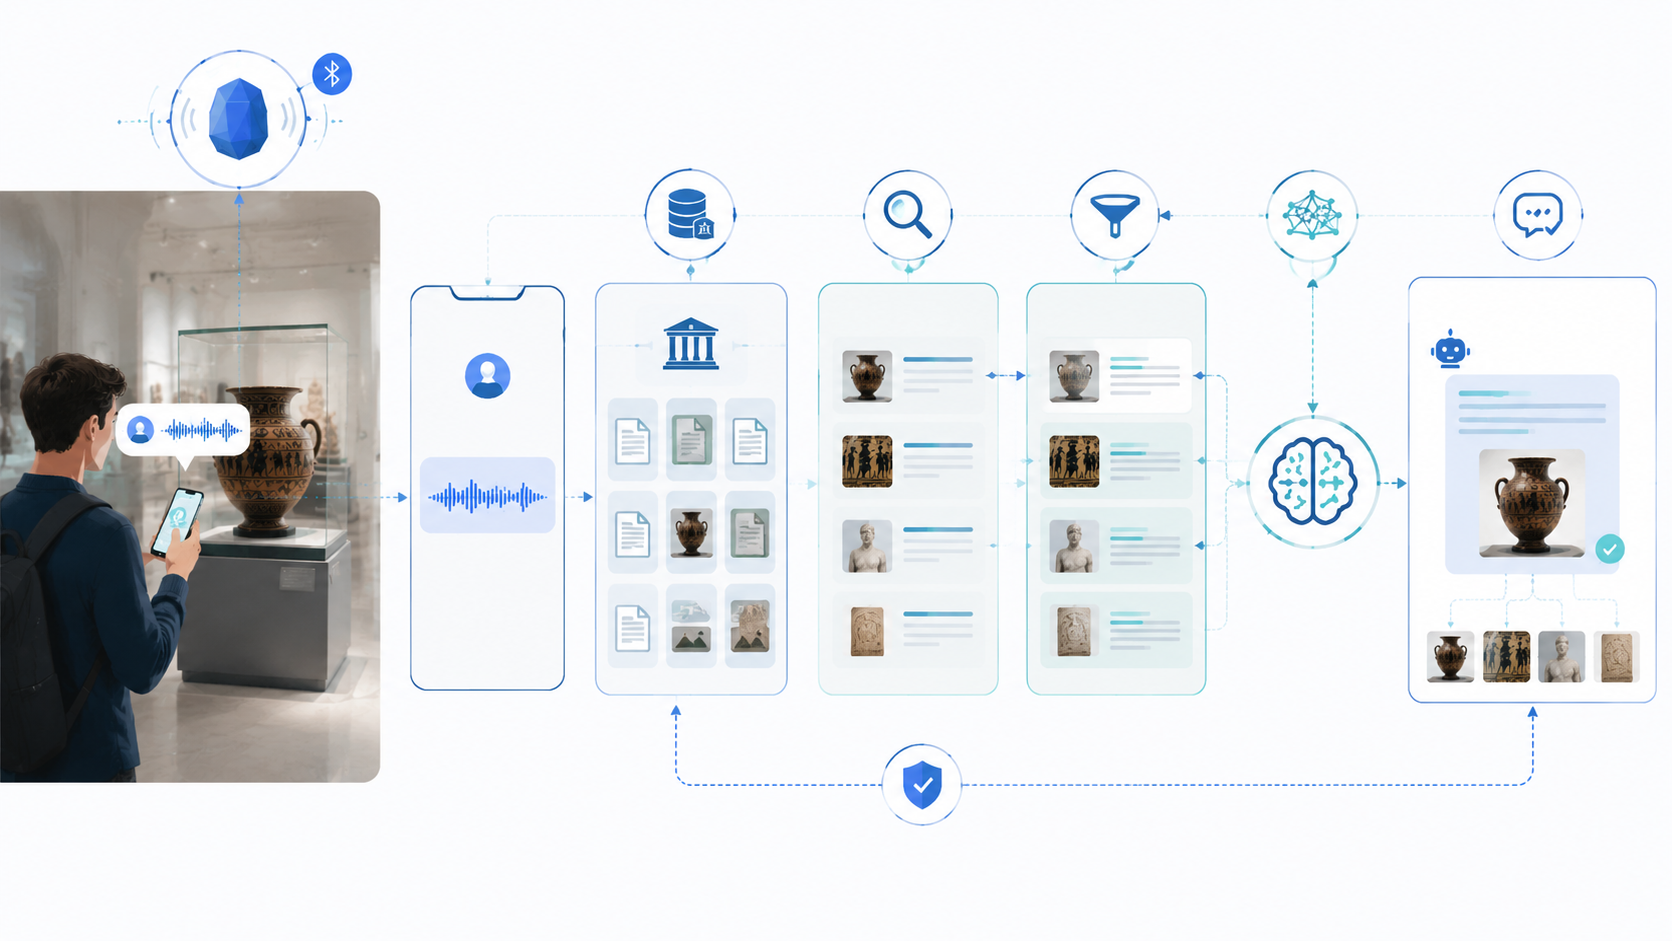
\includegraphics[width=0.92\textwidth]{src/imgs/07/rag-museiq.png}
    \caption[Recuperación aumentada de información en MuseIQ]{Esquema conceptual del uso de RAG para recuperar fragmentos curatoriales relevantes antes de generar una respuesta al visitante. Fuente: elaboración propia con apoyo de generación asistida por IA.}
    \label{fig:rag-museiq}
\end{figure}

La Figura~\ref{fig:rag-museiq} representa con claridad esta secuencia: la pregunta del usuario activa un proceso previo de recuperación documental que condiciona la respuesta final del sistema y mejora su trazabilidad.

\subsection{Corpus curatorial y representación del conocimiento}

La eficacia de RAG depende de la calidad del corpus sobre el que opera. En MuseIQ, dicho corpus está compuesto por contenidos curatoriales institucionales: textos interpretativos, fichas de piezas, descripciones de salas, metadatos de colección y materiales educativos. Este corpus constituye la fuente de conocimiento del sistema y, por lo tanto, debe digitalizarse, organizarse y mantenerse con criterios de control de versiones, consistencia temática y trazabilidad.

En el ámbito del patrimonio cultural existen marcos conceptuales que subrayan la importancia de estructurar adecuadamente la información cultural para facilitar integración, intercambio y reutilización. MuseIQ no necesita implementar por completo una ontología patrimonial compleja en esta etapa, pero sí adopta el principio de que el conocimiento museístico debe mantenerse como recurso institucional gobernado, no como simple texto libre. Esta consideración es clave porque permite filtrar, recuperar y justificar respuestas dentro de límites curatoriales explícitos~\cite{unescoaiculture2025}.

\begin{figure}[!ht]
    \centering
    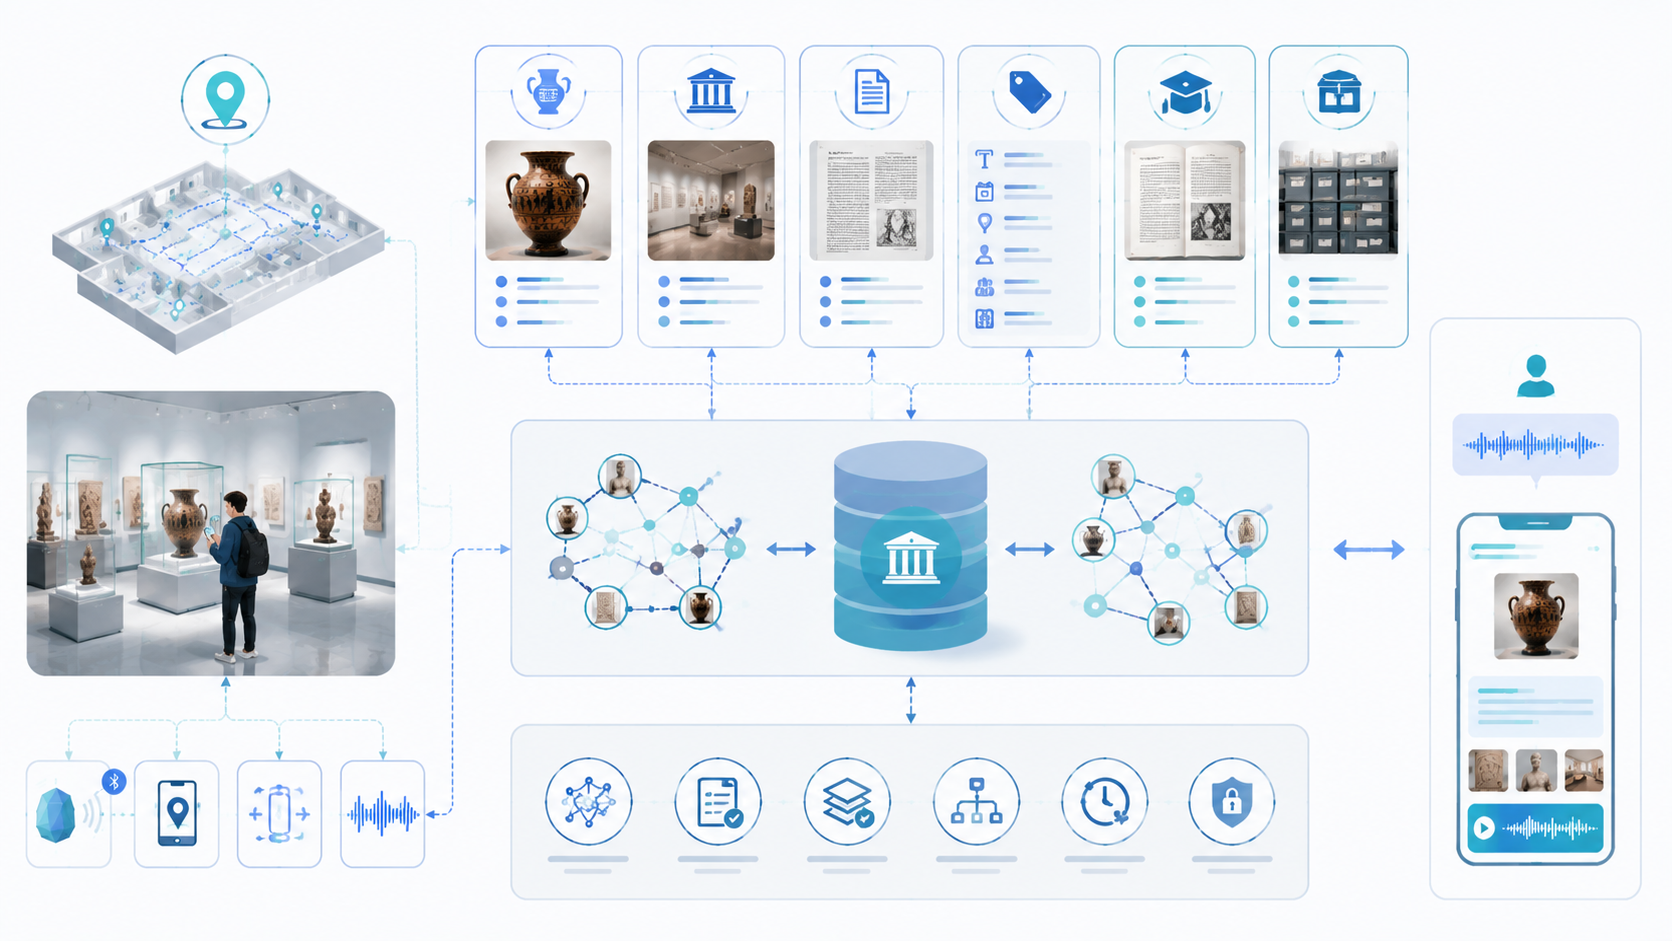
\includegraphics[width=0.92\textwidth]{src/imgs/07/corpus-curatorial.png}
    \caption[Corpus curatorial y organización del conocimiento]{Representación del corpus curatorial institucional como base estructurada de conocimiento para recuperación, trazabilidad y generación de respuestas contextualizadas. Fuente: elaboración propia con apoyo de generación asistida por IA.}
    \label{fig:corpus-curatorial}
\end{figure}

La Figura~\ref{fig:corpus-curatorial} ilustra que el valor del corpus no reside únicamente en almacenar información, sino en organizarla de manera recuperable y coherente con las relaciones entre salas, piezas y contenidos curatoriales.

\subsection{Ventajas y riesgos de la inteligencia artificial en MuseIQ}

La incorporación de IA ofrece ventajas claras para MuseIQ: mayor flexibilidad conversacional, posibilidad de responder consultas abiertas, adaptación a distintas formas de preguntar y mejora de la experiencia interpretativa. No obstante, también introduce riesgos. El más importante es la alucinación, es decir, la generación de respuestas plausibles pero incorrectas. También deben considerarse problemas de gobernanza del contenido, control de fuentes y coherencia con narrativas institucionales.

Por estas razones, la elección tecnológica no puede justificarse únicamente por novedad o capacidad generativa. Su valor para MuseIQ depende de estar acotada por RAG, por un corpus institucional bien definido y por políticas de respuesta compatibles con un dominio patrimonial. En este punto, la tecnología no reemplaza la curaduría, sino que la amplifica mediante una capa de acceso conversacional y contextual.

\begin{figure}[!ht]
    \centering
    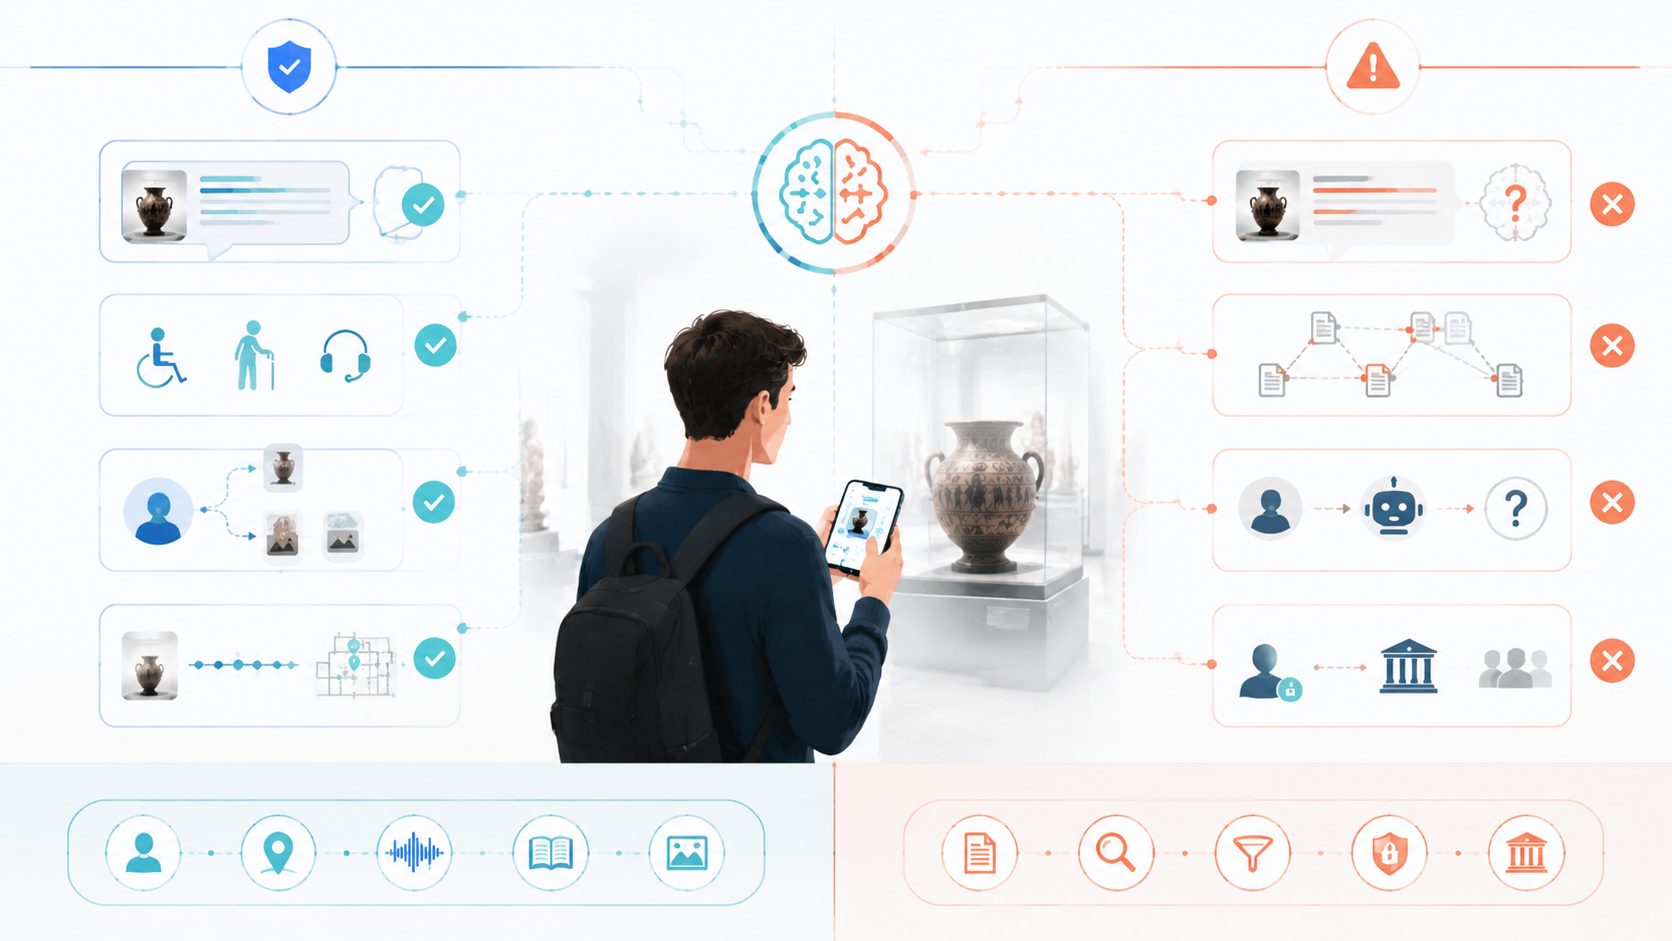
\includegraphics[width=0.92\textwidth]{src/imgs/07/ventajas-riesgos-ia.png}
    \caption[Ventajas y riesgos de la inteligencia artificial en MuseIQ]{Composición comparativa de beneficios y riesgos asociados al uso de inteligencia artificial en una guía museística contextual y conversacional. Fuente: elaboración propia con apoyo de generación asistida por IA.}
    \label{fig:ventajas-riesgos-ia}
\end{figure}

Como resume la Figura~\ref{fig:ventajas-riesgos-ia}, la incorporación de IA ofrece beneficios significativos para accesibilidad y personalización, pero solo resulta defendible si se acompaña de mecanismos de control semántico, trazabilidad y gobernanza institucional.

\section{Criterios de selección e implicancias tecnológicas}

\subsection{Ventajas de la selección tecnológica}

La selección tecnológica de MuseIQ presenta cuatro ventajas principales. La primera es la viabilidad económica: BLE con ESP32 y BYOD reduce inversión inicial en hardware propietario y facilita despliegue incremental. La segunda es la escalabilidad: las tecnologías elegidas permiten ampliar cobertura por salas, actualizar contenidos sin rediseñar toda la infraestructura y adaptar la solución a distintos tipos de institución. La tercera es la accesibilidad funcional: la combinación de smartphone, TTS y STT mejora autonomía del visitante y permite múltiples formas de acceso al contenido. La cuarta es la trazabilidad del conocimiento: RAG y corpus curatorial institucional reducen dependencia de respuestas generativas libres y refuerzan control semántico.

Estas ventajas no eliminan las limitaciones técnicas ya señaladas, como variabilidad de RSSI, heterogeneidad de dispositivos o riesgo de alucinación. No obstante, la combinación elegida es adecuada precisamente porque reconoce esas limitaciones y diseña alrededor de ellas, privilegiando reconocimiento funcional, interacción robusta y control documental antes que precisión extrema o automatización opaca.

\subsection{Limitaciones y consideraciones de implementación}

La selección tecnológica también introduce restricciones que deben reconocerse desde esta etapa. BLE con RSSI presenta variabilidad según obstáculos, orientación del dispositivo y condiciones del entorno. El enfoque BYOD implica diversidad de hardware, sensores y políticas de permisos. Las tecnologías de voz dependen de condiciones acústicas razonables y de una experiencia de uso bien resuelta. Finalmente, la capa basada en modelos de lenguaje exige control riguroso del corpus, de la recuperación y de los criterios de respuesta para no comprometer precisión curatorial.

Estas limitaciones no invalidan la propuesta, pero sí condicionan sus decisiones de diseño. En lugar de buscar máxima precisión geométrica o autonomía total de la IA, MuseIQ se apoya en tecnologías cuya madurez y costo permiten una implementación gradual y verificable. Por ello, la siguiente etapa del desarrollo debe traducir estas decisiones tecnológicas en estructuras de datos, reglas de inferencia, componentes de software y mecanismos de despliegue coherentes con esas restricciones.

\subsection{Proyección hacia los capítulos siguientes}

La base tecnológica aquí descrita condiciona de forma directa los capítulos siguientes de la tesis. En el diseño de datos de entrada será necesario formalizar el esquema del corpus curatorial, su segmentación y sus relaciones con salas, piezas y zonas. En el diseño y despliegue del sistema se deberá especificar la arquitectura de comunicación entre aplicación móvil, servicios de backend, capa de recuperación y módulo conversacional. Finalmente, en la implementación y validación será imprescindible definir estrategias de calibración de beacons, reglas de inferencia contextual, control de permisos y métricas de desempeño técnico y de experiencia de usuario.

En consecuencia, este capítulo no agota el detalle ingenieril de la solución, pero sí establece con claridad qué tecnologías sostienen MuseIQ y por qué su combinación resulta defendible dentro de una tesis de ingeniería aplicada orientada al contexto museístico peruano.
